% ==============================================================================
% ================================ AUFGABE 2 ===================================
% ==============================================================================

%\chapter{Aufgabe 2: Mealy-Automat}
%\label{chap:aufgabe2}
%\thispagestyle{fancy}

\section{Aufgabe 2: Mealy-Automat}
So wie Fleury, M. Otten \cite{2} es erläutert, wird in diesem Kapitel ein Mealy-Automat als Paritäts-Prüfer für eine serielle 3-Bit-Folge entworfen. 
Der Automat prüft fortlaufend, ob die Anzahl der High-Pegel (\textit{1}) in der aktuellen 3-Bit-Folge ungerade ist. 
Tritt dieser Fall ein, wird am synchronisierten Ausgang \( A_S \) unmittelbar ein High-Pegel ausgegeben.

Zunächst erfolgt der Entwurf mit sieben Zuständen \( Z_1 \) bis \( Z_7 \). 
Anschließend wird der Automat durch Eliminierung redundanter Zustände auf fünf Zustände optimiert.

\subsection{Entwurf mit sieben Zuständen}
Die Zustände repräsentieren die Anzahl der bereits eingelesenen Bits sowie die Parität dieser Bits.
\begin{itemize}
    \item \( Z_1 \): 0 Bit eingelesen, Parität gerade (\textit{0})
    \item \( Z_2 \): 1 Bit eingelesen, Parität gerade (\textit{0})
    \item \( Z_3 \): 1 Bit eingelesen, Parität ungerade (\textit{1})
    \item \( Z_4 \): 2 Bit eingelesen, Parität gerade (\textit{0})
    \item \( Z_5 \): 2 Bit eingelesen, Parität ungerade (\textit{1})
    \item \( Z_6 \): 3 Bit eingelesen, Parität gerade (\textit{0}) – Ausgang \( A = 0 \)
    \item \( Z_7 \): 3 Bit eingelesen, Parität ungerade (\textit{1}) – Ausgang \( A = 1 \)
\end{itemize}
Die Zustandsübergänge werden durch den Eingangsvektor \( E \) (\textit{serielles Bit}) gesteuert. 
Der Ausgang \( A \) gibt an, ob die Parität der vollständigen 3-Bit-Folge ungerade ist.
\subsubsection{Zustandsübergangstabelle für sieben Zustände}
\begin{table}[H]
\centering
\begin{tabular}{c|c|c|c}
\toprule
\textbf{Z} & \textbf{E} & \textbf{A} & \textbf{Z$_{\text{next}}$} \\
\midrule
\( Z_1 \) & 0 & 0 & \( Z_2 \) \\
\( Z_1 \) & 1 & 0 & \( Z_3 \) \\
\( Z_2 \) & 0 & 0 & \( Z_4 \) \\
\( Z_2 \) & 1 & 0 & \( Z_5 \) \\
\( Z_3 \) & 0 & 0 & \( Z_5 \) \\
\( Z_3 \) & 1 & 0 & \( Z_4 \) \\
\( Z_4 \) & 0 & 0 & \( Z_6 \) \\
\( Z_4 \) & 1 & 0 & \( Z_7 \) \\
\( Z_5 \) & 0 & 0 & \( Z_7 \) \\
\( Z_5 \) & 1 & 0 & \( Z_6 \) \\
\( Z_6 \) & 0 & 0 & \( Z_2 \) \\
\( Z_6 \) & 1 & 0 & \( Z_3 \) \\
\( Z_7 \) & 0 & 1 & \( Z_2 \) \\
\( Z_7 \) & 1 & 1 & \( Z_3 \) \\
\bottomrule
\end{tabular}
\caption{Zustandsübergangstabelle mit sieben Zuständen (\textit{Quelle: Eigene Darstellung})}
\label{tab:mealy_7states}
\end{table}
\begin{figure}[H]
\centering
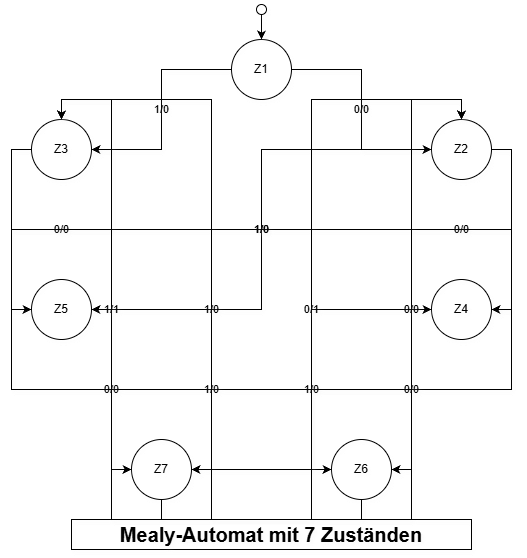
\includegraphics[width=0.44\textwidth]{asset/image/Aufgabe2.png}
\caption{Zustandsgraph des Mealy-Automaten mit sieben Zuständen (\textit{Quelle: Eigene Darstellung})}
\label{fig:mealy7}
\end{figure}
\subsection{Optimierung auf fünf Zustände}
Die Zustände \( Z_6 \) und \( Z_7 \) erfüllen lediglich die Funktion, den Ausgang für die dritte Bitposition 
bereitzustellen. Da es sich um einen Mealy-Automaten handelt, kann der Ausgang jedoch bereits 
in den Zuständen \( Z_4 \) und \( Z_5 \) in Abhängigkeit vom aktuellen Eingangsbit \( E \) gebildet werden. 
Dadurch werden \( Z_6 \) und \( Z_7 \) redundant und können entfallen.
\subsubsection{Optimierte Zustandsdefinition}
Die verbleibenden fünf Zustände sind:
\begin{itemize}
    \item \( Z_1 \): 0 Bit eingelesen, Parität gerade (\textit{Startzustand})
    \item \( Z_2 \): 1 Bit eingelesen, Parität gerade
    \item \( Z_3 \): 1 Bit eingelesen, Parität ungerade
    \item \( Z_4 \): 2 Bit eingelesen, Parität gerade
    \item \( Z_5 \): 2 Bit eingelesen, Parität ungerade
\end{itemize}
Der Ausgang wird nun direkt in \( Z_4 \) und \( Z_5 \) beim Übergang zum nächsten Zustand 
(\textit{also beim dritten Bit}) gebildet.
\begin{figure}[H]
\centering
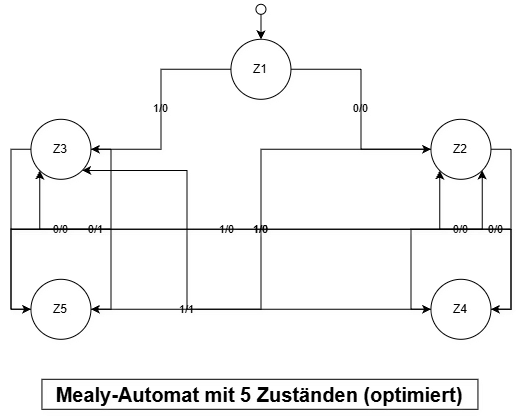
\includegraphics[width=0.44\textwidth]{asset/image/Aufgabe2II.png}
\caption{Zustandsgraph des optimierten Mealy-Automaten mit fünf Zuständen (\textit{Quelle: Eigene Darstellung})}
\label{fig:mealy5}
\end{figure}
\subsubsection{Zustandsübergangstabelle für fünf Zustände}
\begin{table}[h]
\centering
\begin{tabular}{c|c|c|c}
\toprule
\textbf{Z} & \textbf{E} & \textbf{A} & \textbf{Z$_{\text{next}}$} \\
\midrule
\( Z_1 \) & 0 & 0 & \( Z_2 \) \\
\( Z_1 \) & 1 & 0 & \( Z_3 \) \\
\( Z_2 \) & 0 & 0 & \( Z_4 \) \\
\( Z_2 \) & 1 & 0 & \( Z_5 \) \\
\( Z_3 \) & 0 & 0 & \( Z_5 \) \\
\( Z_3 \) & 1 & 0 & \( Z_4 \) \\
\( Z_4 \) & 0 & 0 & \( Z_2 \) \\
\( Z_4 \) & 1 & 1 & \( Z_3 \) \\
\( Z_5 \) & 0 & 1 & \( Z_3 \) \\
\( Z_5 \) & 1 & 0 & \( Z_2 \) \\
\bottomrule
\end{tabular}
\caption{Zustandsübergangstabelle mit fünf Zuständen (\textit{optimiert}) (\textit{Quelle: Eigene Darstellung})}
\label{tab:mealy_5states}
\end{table}
\subsubsection{Ergebnis der Optimierung}
Durch die Verlagerung der Ausgangslogik in die Zustände \( Z_4 \) und \( Z_5 \) 
konnten die beiden Zustände \( Z_6 \) und \( Z_7 \) vollständig eliminiert werden. 
Der optimierte Mealy-Automat arbeitet mit \textbf{fünf Zuständen} und erfüllt 
die gleiche Spezifikation wie der ursprüngliche Automat mit sieben Zuständen. \hspace{4cm} \[\boxed{ \text{Optimierte Zustandsanzahl: } 5 }\]

% ==============================================================================
% ================================ AUFGABE 2 ===================================
% ==============================================================================